\chapter{Query Facet Extraction}
\label{ch:facet}
\section{Introduction}
In conventional faceted search, facets are typically generated in advance for an entire corpus~\cite{stoica2007automating,dakka2008automatic} either manually or semi-automatically, and then recommended for particular queries. However, this approach is difficult to extend to faceted web search due to the large and heterogeneous nature of the web~\cite{teevan2008challenges}: because the web is very large, it is
difficult to assign quality facets to every document in the collection and to retrieve the full set of search results and their associated facets at query time; and because the web is heterogeneous, it is difficult to apply the same facets to every search result or every query.

To cope with this challenge, in this chapter, we propose an alternative solution, called \textbf{query facet extraction}, which extracts facets for queries from their web search results. For example, when users search with the query \concept{baggage allowance}, the system might extract query facets like airlines, \{\concept{Delta}, \concept{JetBlue}, \concept{AA}, ...\}, travel classes, \{\concept{first}, \concept{business}, \concept{economy}\}, and flight types, \{\concept{international}, \concept{domestic}\}. Changing from a global approach that generates facets in advance for an entire corpus to a query-based approach that extract facets from the top-ranked search results, query facet extraction appears to be a promising direction for solving the open-domain faceted search problem -- it not only make the facet generation problem easier, but also addresses the facet recommendation problem at the same time.


We define a \textbf{query facet} as a set of coordinate terms (\eg, \{\concept{AA}, \concept{Delta}, \concept{JetBlue},...\}) that explicitly represent one aspect (\eg, \concept{airlines}) of its query (\eg, \concept{baggage allowance}). The coordinate terms share a semantic relationship by being grouped under a more general hypernym (``is a'' relationship, \eg, \concept{AA}, \concept{Delt}, \concept{JetBlue} are all \concept{airlines}). 
% Terms in query facet are generally called \textbf{facet terms}. When it is clear from context, we will simply use ``facet'' for ``query facet'', and ``term'' for ``facet term'' for convenience. Based on these definitions, \textbf{query facet extraction} is to extract query facets for a given query from certain resources, and in our case the top search results for that query.
In Table~\ref{tab:facet-facetexample}, we show query facets for three example queries. We will using the first query \concept{Mars landing} as example for explanation. For the first query, the first query facet, \{\textit{Curiosity}, \textit{Opportunity}, \textit{Spirit}\}, includes different Mars rovers. The second query facet, \{\textit{USA}, \textit{UK}, \textit{Soviet Union}\}, includes countries relevant to Mars landings. These are both facets where the terms are instances of the same semantic class. 
Somewhat differently, the last facet, \{\textit{video}, \textit{pictures}, \textit{news}\}, includes labels for different query subtopics. These labels can be viewed as instances of a special semantic class, the subtopics of the query \textit{mars landing}. 
\begin{table}[ht!]
\centering
\caption{Query facet examples for three queries}
\label{tab:facet-facetexample}
\begin{tabular}{|l|} \hline
Query 1: Mars landing \\\hline
Query Facet 1: Curiosity, Opportunity, Spirit \\
Query Facet 2: USA, UK, Soviet Union \\
Query Facet 3: video, pictures, news \\\hhline{|=|}
Query 2: baggage allowance \\\hline
Query Facet 1: AA, Delta, Jetblue,  ... \\
Query Facet 2: international, domestic \\
Query Facet 3: first class, business class, economy class \\
Query Facet 4: weight, size, quantity \\\hhline{|=|}
Query 3: Mr Bean \\\hline
Query Facet 1: comics, movies, tv, books \\
Query Facet 2: The Curse of Mr Bean, Mr Bean Goes to Town, ...\\
Query Facet 3: Rowan Atkinson, Richard Wilson, Jean Rochefort,  ...\\ 
Query Facet 4: Mr Bean, Irma gobb, Rupert, Hubert, ...\\\hline
\end{tabular}
\end{table}


In this work, we use query facet extraction to address the problem of facet generation in Faceted Web Search. This approach first extracts candidate facets from the top search results based on textual and HTML patterns, and then refines the extracted candidates, which are often very noisy, using clustering methods. We develop a supervised method based on a graphical model for refining facet candidates. The graphical model learns how likely it is that a term should be selected from the candidates and how likely it is that two terms should be grouped together in a query facet. Further, the model captures the dependencies between the two factors. We propose two algorithms for approximate inference on the graphical model since  exact inference is intractable. This proposed method can easily incorporate a rich set of features and learn from available human labels.
%Also, we design an evaluation metric for query facet extraction, which combines recall and precision of the facet term, with the grouping quality.
%The evaluation metrics will be discussed in Chapter~\ref{ch:intrinsiceval}.

The rest of this chapter is organized as follows. We first define the task of query facet extraction and related concepts in Section~\ref{sec:facet-task}, and then describe a general framework to solve this problem in Section~\ref{sec:facet-framework}. We propose a supervised clustering method based on a graphical model for refining extracted candidates in Section~\ref{sec:facet-gm}. Last, we describe other methods that can be used for refining extracted candidates, including topic modeling (e.g., pLSA, LDA) and a variation of quality threshold clustering model~\cite{dou2011finding} in Section~\ref{sec:facet-other}. 
%The work in this chapter is completed and published~\cite{kong2013extracting}.

\section{Task Description}
\label{sec:facet-task}
\subsection{Query Facet}
To differentiate our work with facets in conventional faceted search, we call typically facets for a particular query ``query facets''. A query facet is a set of coordinate terms -- i.e., terms that share a semantic relationship by being grouped under a more general hypernym (``is a'' relationship), and they succinctly represent different options in the same category that a user can select to refine the issued query. This definition of query facets corresponds to one-level taxonomies in faceted taxonomy, in which only information objects that belong to a same parent node are shown as a query facet. We leave generating query facets as two or more level taxonomies in future work.

\subsection{Facet Term}
We call the terms inside facets ``facet terms'', which can be single words (e.g. \concept{international}, \concept{domestic} in Table~\ref{tab:facet-facetexample}) or phrases (e.g. \concept{first class}, \concept{business class} in Table~\ref{tab:facet-facetexample}). 
These facet terms can be instances of a semantic class, for example \concept{Curiosity}, \concept{Opportunity}, \concept{Spirit} are all Mars rovers. They can be labels for query subtopics, such as \concept{video}, \concept{pictures}, \concept{news} for the query \concept{mars landing}. Facet terms of a query succinctly represent different options in the same category that a user can select to refine the issued query. 

When it is clear from context, we will simply use ``facet'' for ``query facet'', and ``term'' for ``facet term'' for convenience.

\subsection{Query Facet Extraction}
Based on the definitions above, query facet extraction is to extract query facets for a given query from certain resources. While a variety of different resources can be used for query facet extraction, such as a query log, anchor text, taxonomy and social folksonomy, In this work, we only focus on extracting query facets from the top ranked web search results, and and leave others as future work.

\section{General Framework}
\label{sec:facet-framework}
In this section, we describe the general framework we use for extracting query facet from web search results. It generally works as follows: (1) Given a query, retrieve the top search results. (2) Extract candidate facets from the search results based on pre-defined extraction patterns. (3) Refine the candidates to final query facets by re-clustering facets or facet terms in the candidate set. Step 2 and 3 are further described below.

\subsection{Candidate Extraction} 
\label{sec:extractCandidateLists}
Following \citet{dou2011finding}, we use pattern-based semantic class extraction approach~\cite{shi2010corpus} to extract lists of coordinate terms from search results as candidates for query facets.
In pattern-based semantic class extraction, patterns are applied on the corpus to discover specific relationships between terms.
For example, the pattern ``\textit{NP} such as \textit{NP}, \textit{NP}, ..., and \textit{NP}'' can be used to extract coordinate terms and their hypernyms from text.
Besides lexical patterns, HTML patterns are often used on HTML documents to extract coordinate terms from some HTML structures, like <UL>, <SELECT> and <TABLE>.
\begin{table}[ht!]
\centering
\caption{Semantic class extraction patterns}
\label{tab:patterns}
\begin{tabular}{|c|l|} \hline
Type& Pattern\\ \hline
Lexical & \textit{item}, \{,\textit{item}$\}^*$, (and|or) \{other\} \textit{item} \\  \hline
\multirow{4}{*}{HTML}
& <select><option>\textit{item}</option>...</select>\\\cline{2-2}
& <ul><li>\textit{item}</li>...</ul>\\\cline{2-2}
& <ol><li>\textit{item}</li>...</ol>\\\cline{2-2}
& <table><tr><td>\textit{item}<td>...</table>\\ \hline
\end{tabular}
\end{table}

\todo{Why these patterns}
We use both of the two types of patterns, summarized in Table~\ref{tab:patterns}.
In the table, all \textit{items} in each pattern are extracted as a candidate list.
For example, from the text sentence ``\textit{... Mars rovers such as Curiosity, Opportunity and Spirit}'', 
according to the lexical pattern, we will extract a candidate list \{\textit{Curiosity}, \textit{Opportunity}, \textit{Spirit}\}.
For the lexical pattern, we also restrict those \textit{items} to be siblings in the parse tree of that sentence.
We use the PCFG parser~\cite{klein2003accurate}
implemented in Stanford CoreNLP\footnote{http://nlp.stanford.edu/software/corenlp.shtml} for parsing documents.

HTML lists \textit{UL} and \textit{OL} can be nested, as shown in Figure~\ref{fig:nestedlist}. For nested HTML lists, we extract all the sibling items. For the example in Figure~\ref{fig:nestedlist}, we will extract two lists,
\{\concept{Coffee}, \concept{Tea}, \concept{Milk}\} and \{\concept{Black tea}, \concept{Green tea}\}.
For HTML tables, following Dou et al.~\cite{dou2011finding}, lists from each column and each row are extracted.

\begin{figure}[ht!]
\centering
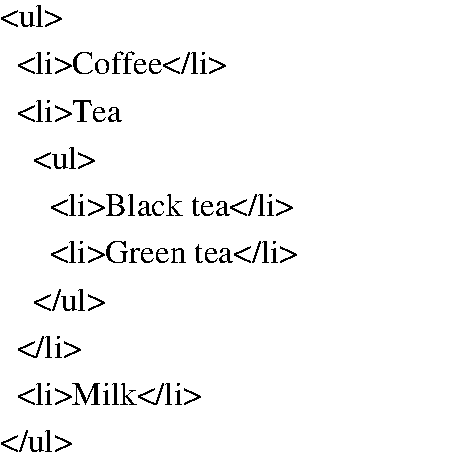
\epsfig{file=drawing/nestedHtmlList.pdf,scale=0.7}
\caption{An example for nested HTML lists.}
\label{fig:nestedlist}
\end{figure}

After extracting the candidates from the top ranked search results, we further clean them as follows.
First, all the list items are normalized by converting text to lowercase and removing non-alphanumeric characters.
Then, we remove stopwords and duplicate items in each lists.
Finally, we discard all lists that contain only one item or more than 200 items. 

After the cleaning process, we harvest a set of query facet candidates, which we call \textbf{candidate lists}. We name terms in a candidate list \textbf{list items}, in order to differentiate with facet terms (\ie, terms in a query facet).
%$\mathcal{L}=\{L\}$, where each list $L=\{t\}$ is a set of list items.

\subsection{Facet Refining}
\label{sec:facet-refine}
The candidate lists extracted are usually noisy~\cite{zhang2009employing},
and could be non-relevant to the issued query, therefore they cannot be used directly as query facets. For example, Table~\ref{tab:candidates} shows four candidate lists extracted for the query \concept{baggage allowance}. $L_1$ contains terms that are relevant to \concept{baggage allowance}, but they are not coordinate terms -- \concept{delta}, \concept{france} and \concept{round-trip} are not members of the same class. 
$L_2$ is a valid query facet, but it is incomplete -- another airline \concept{aa} appears in $L_3$. $L_3$ is mixed with different facets, airlines and travel classes. $L_4$ is non-relevant to the query. 
\begin{table}[ht!]
\centering
\caption{Four candidate lists for the query \concept{baggage allowance}}
\label{tab:candidates}
\begin{tabular}{|l|} \hline
 %Candidate facets \\ \hline
$L_1$: delta, france, round-trip\\
$L_2$: delta, jetblue, british airways\\ 
$L_3$: aa, first, business, economy\\
$L_4$: hard to remember, playing it by ear, ...\\
\hline
\end{tabular}
\end{table}

Since the candidate lists are frequently noisy, we need an effective way to refine extracted candidate lists into high-quality query facets. The facet refining problem can be essentially viewed as a \emph{selective} clustering problem, in which noisy terms are discarded, and facet terms (\eg, \concept{aa}, \concept{delta}, \concept{jetblue}, \concept{british airways}, \concept{first}, \concept{business} and \concept{economy}) are selected, then clustered into query facets (\eg, \{\concept{aa}, \concept{delta}, \concept{jetblue}, \concept{british airways}\} and \{\concept{first}, \concept{business},\concept{economy}\}). 
Facet refining is the core problem of query facet extraction. Existing models differ in how they refine candidate lists. To address this problem, we develop a supervised method based on a graphical model, which will be presented in the next section.


\section{Query Faceting Models}
\label{sec:facet-gm}
In this section, we describe query faceting (QF) models, our supervised methods based on a directed graphical model for facet refining. A directed graphical model (or Bayesian network) is a graphical model that compactly represents a probability distribution over a set of variables ~\cite{pearl1988probabilistic}. It consists of two parts: 1) a directed acyclic graph in which each vertex represents a variable, and 2) a set of conditional probability distributions that describe the conditional probabilities of each vertex given its parents in the graph.

We treat facet refining as a selective clustering problem (as described in Section~\ref{sec:facet-refine}), and solve it as a labeling problem, in which we are trying to predict 1) whether a list item is a facet term, and 2) whether a pair of list items is in a same query facet. Then, we used a directed graphical model to exploit the dependences that exist between those labels. Similar to conditional random fields~\cite{lafferty2001conditional}, we directly model the conditional probability $P(y|x)$, where $y$ is the label we are trying to predict and $x$ is the observed data -- list items and item pairs. Thus, it avoids modeling the dependencies among the input variables $x$, and can handle a rich set of features. For our graph model, exact maximum a posteriori inference is intractable; therefore, we approximate the results using two algorithms.

In the rest of this section, we will first describe the facet refining problem more formally in Section~\ref{sec:facet-formulation}, and then present our graphical model in Section~\ref{sec:facet-model}. We will describe how to train and perform inference on the model in Section~\ref{sec:facet-train} and Section~\ref{sec:facet-infer} respectively.

\subsection{Problem Formulation}
\label{sec:facet-formulation}
Before diving into the QF method, we first define the facet refining problem more formally. We use $F=\{t_i\}$ to denote a query facet, consisted by a set of facet terms $t_i$. $\mathcal{F}=\{F_i\}$ denotes the set of query facets for the given query. $T_\mathcal{F}=\bigcup_i{F_i}$ denotes all the facet terms in $\mathcal{F}$. Candidate lists (or candidate facets) are just an imperfect version of query facets, and we substitute ``F'' with ``L'' to denote corresponding variables. $L=\{t_i\}$ denotes a candidate list. $\mathcal{L}=\{L_i\}$ denotes all the candidate lists extracted for the query. $T_\mathcal{L}=\bigcup_i{L_i}$ denotes all list items (or terms) in the candidate lists. Based on the formulation, the facet refining problem is simply to find $\mathcal{F}$ constrained with $T_\mathcal{F} \subseteq T_\mathcal{L}$, given $\mathcal{L}$ (and possibly other resources).

In our query faceting models, facet refining problem was treated as a label prediction problem. It aims to learn and predict jointly 1) whether a list item is a facet term and 2) whether a pair of list items are in the same query facet. We denote the two types of labels as follows. The term/item labels are denoted by $Y=\{y_i\}$, where $y_i = 1\{t_i\!\in\! T_{\mathcal{F}}\}$ is a label indicating whether a list item $t_i$ is indeed a facet term. Here $1\{\cdot\}$ is an indicator function which takes on a value of 1 if its argument is true, and 0 otherwise. The pair labels are denoted by $Z=\{z_{i,j}\}$, where $z_{i,j} = 1\{\exists\, F\!\in\!\mathcal{F}, \, t_{i}\!\in\!F  \wedge  t_{j}\!\in\!F \}$ is a label indicates whether list item $t_i$ and $t_j$ are in a same query facet. Thus, the facet refining problem is now formulated as the problem of predicting labels $Y$ and $Z$.

\subsection{The Graphical Model}
\label{sec:facet-model}
Our supervised method is based on a directed graphical model, aiming to capture the dependencies between the term and pair labels. The graphical model is shown in Figure~\ref{fig:gm}. We further describe it as follows.

\begin{figure}[ht!]
\centering
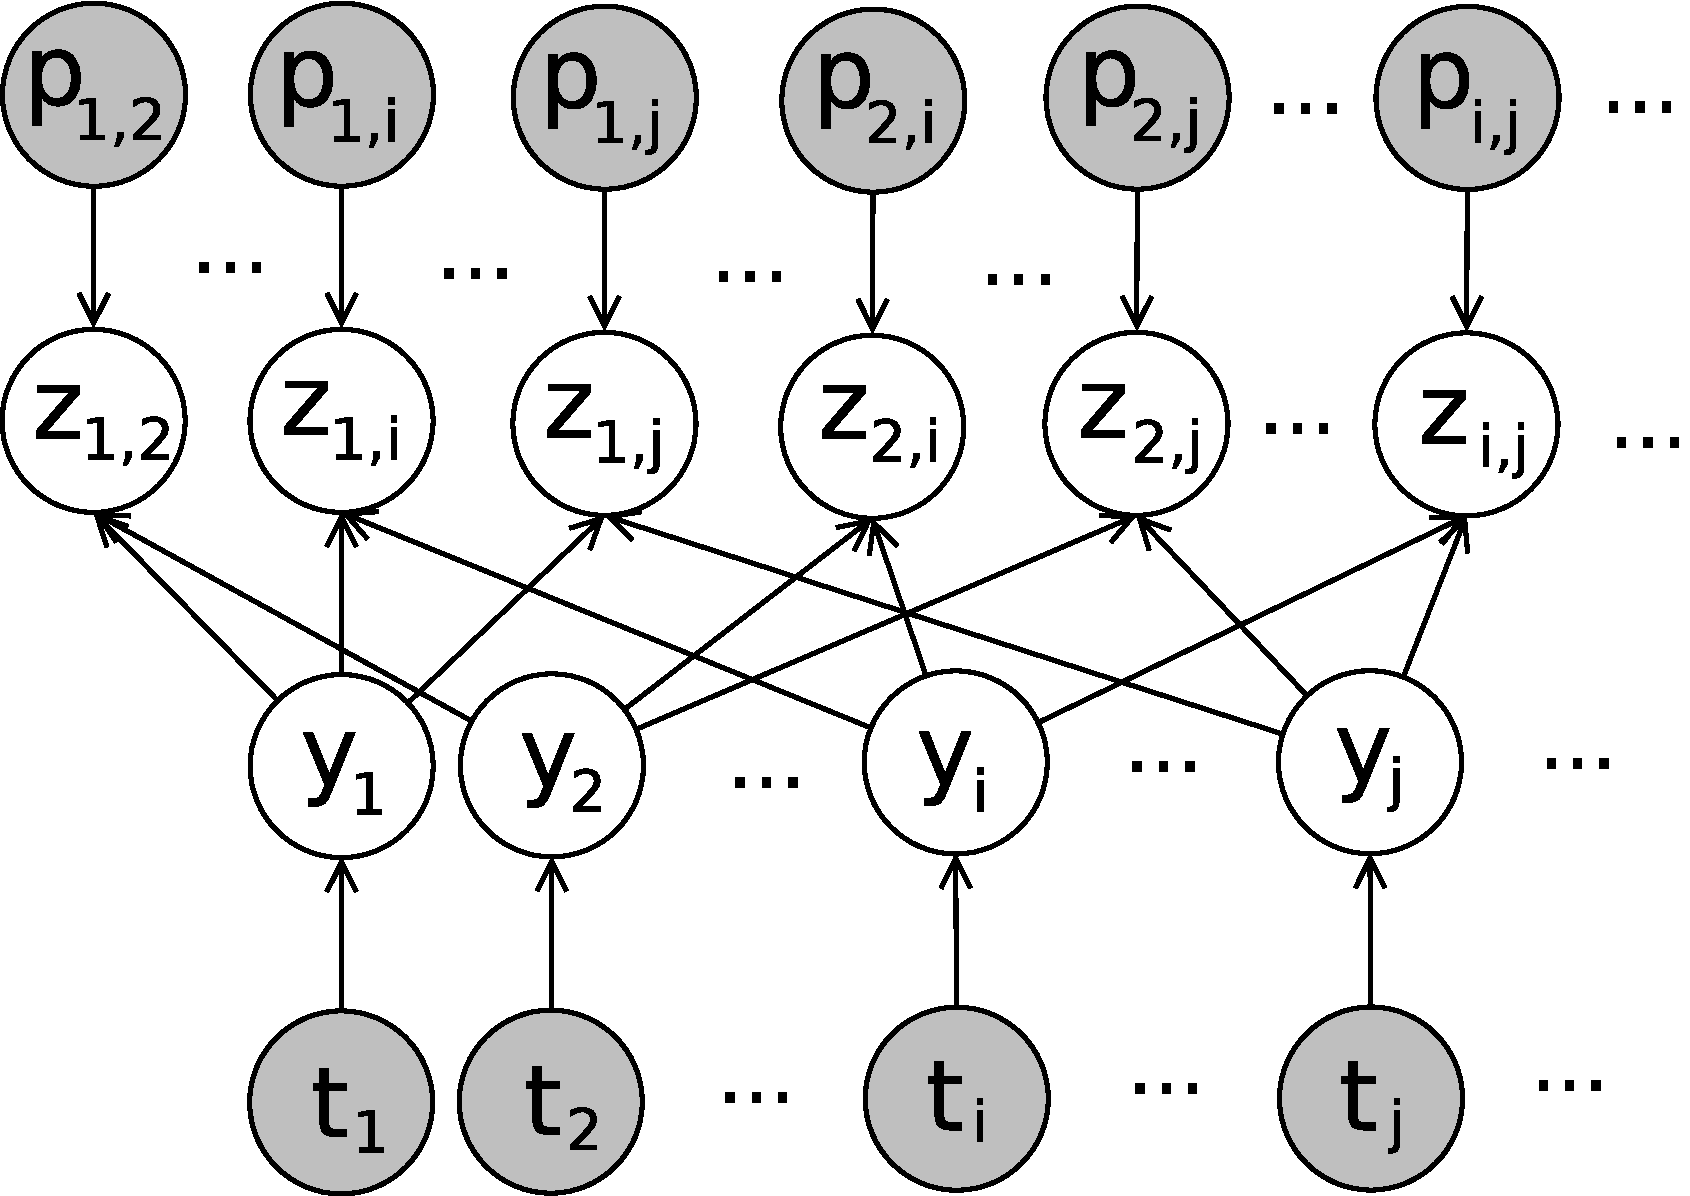
\epsfig{file=drawing/gm.pdf,scale=0.20}
\caption{A graphical model for candidate list data}
\label{fig:gm}
\end{figure}

\subsubsection{The Graph}
First, we describes the four types of variables in the graphical model as follows. We use the formulation described in Section~\ref{sec:facet-formulation}.
\begin{itemize}
 \item list items: $t_i \in T_\mathcal{L}$, as defined before, are all the list items from the extracted candidate lists.
 \item item pairs: $p_{i,j}=(t_i,t_j)$ is simply a short name for term pair $t_i$ and $t_j$. $P_{\mathcal{L}}=\{p_{i,j}|\, t_i,t_j\!\in\!T_{\mathcal{L}}, \, t_i \!\neq\! t_j \}$ are all the item pairs in $T_\mathcal{L}$.
 \item item labels: $y_i \in Y$, as defined before, are all item labels.
  \item pair labels: $z_{i,j} \in Z$, as defined before, are pair labels.
\end{itemize}
List items $t_i$ and item pairs $p_{i,j}$ will be characterized by corresponding features (and will be described in Section~\ref{sec:facet-features}). They are always observed. features (and will be described in Section~\ref{sec:facet-features}). They are always observed. Item labels $y_i$ and pair labels $z_{i,j}$ are what we are trying to predict. In summary, the vertices in our graphical model are $V=T_{\mathcal{L}} \cup P_{\mathcal{L}} \cup Y \cup Z$.

Second, as shown in Figure~\ref{fig:gm}, there are three types of edges in the graph:
\begin{itemize}
 \item edges from each list item $t_i$ to its corresponding labels $y_i$. 
 \item edges that point to each item pair label $z_{i,j}$ from the two corresponding list items $y_i$ and $y_j$.
 \item edges from each item pair $p_{i,j}$ to its corresponding label $z_{i,j}$.
\end{itemize}

\subsubsection{Conditional Probability Distributions}
We use logistic-based conditional probability distributions (CPDs) for variable $y_i$ and $z_{i,j}$, defined as in Equation~\ref{eq:y} and Equation~\ref{eq:z},
\begin{equation}
\label{eq:y}
P(y_i = 1|t_i)=\frac{1}{1+\exp\{-\sum_k{\lambda_k f_k(t_i)}\}},
\end{equation}
\begin{equation}
\label{eq:z}
P(z_{i,j} = 1|p_{i,j},y_i, y_j)=\frac{y_i y_j}{1+\exp\{-\sum_k{\mu_k g_k(p_{i,j})}\}},
\end{equation}
where $f_k$ and $g_k$ are features that characterize a list item and a item pair respectively. $\lambda$ and $\mu$ are the weights associated with $f_k$ and $g_k$ respectively. Compared to a conventional logistic function, Equation~\ref{eq:z} has an extra term, $y_iy_j$, in the numerator. When $y_i=0$ or $y_j=0$, we have $P(z_{i,j}=1|p_{i,j},y_i,y_j)=0$. This means when either of the two list items is not a facet term, the two items can never appear in a query facet together.
When both of the $t_i$ and $t_j$ are facet terms, $P(z_{i,j}=1|p_{i,j},y_i,y_j)$ becomes a conventional logistic function, which models the probability of $t_i$ and $t_j$ being grouped together in a query facet, given the condition that both $t_i$ and $t_j$ are facet term.

\subsubsection{Joint Conditional Probability}
Similar as in conditional random fields~\cite{lafferty2001conditional}, we directly model the joint conditional probability $P(Y,Z|T_{\mathcal{L}},P_{\mathcal{L}})$. Thus, it avoids modeling the dependencies among the input variables $T_{\mathcal{L}},P_{\mathcal{L}}$, and can handle a rich set of features. The joint conditional probability for the graphical model is calculated as
\begin{equation}
\label{eq:joint}
P(Y,Z|T_{\mathcal{L}},P_{\mathcal{L}}) = \prod_{i}{P(y_i|t_i)}\prod_{i,j}{P(z_{i,j}|p_{i,j},y_i, y_j)},
\end{equation}
where the $P(y_i|t_i)$ and $P(z_{i,j}|p_{i,j}, y_i, y_j)$ are defined in Equation~\ref{eq:y} and Equation~\ref{eq:z} respectively.

\subsubsection{Features}
\label{sec:facet-features}
There are two types of features used in our graphical model, summarized in Table~\ref{tab:feature}.

\textbf{Item features}, $f_k(t)$ in the graphical model, characterize a single list item.
To capture the relevance of item $t$ to the query, 
we use some TF/IDF-based features extracted from the top $k$ search results, $\mathcal{D}$.
For example, \textit{snippetDF} is the number of snippets in top $k$ search results that contain item $t$.
\textit{snippetDF} and other frequency-based features are normalized using $log(frequency+1)$.
To capture how likely item $t$ is to be an instance of a semantic class, we use features extracted from candidate lists.
For example, \textit{listTF} is the frequency of $t$ in the candidate lists extracted from $\mathcal{D}$.
Some list items occur frequently in candidate lists across different queries, such as 
\textit{home}, \textit{contact us} and \textit{privacy policy}. They are treated as stopwords, and removed from the candidate lists.
We also use $listIDF$ to cope with this problem. 
$listIDF$ is the IDF of a list item in a general collection of candidate lists we extracted (see Section~\ref{sec:ie-data}).
It is calculated as $listIDF(t)=\log{\frac{N-N_{t}+0.5}{N_t+0.5}}$, where $N$ is the total number of lists in the collection, 
$N_t$ is the number of lists contain $t$.
The same form is used for \textit{clueIDF}, IDF in ClueWeb09\footnote{http://lemurproject.org/clueweb09} collection.

\textbf{Item Pair Features}, $g(p_{i,j})$ in the graphical model, 
are used to capture how likely a pair of list items should be grouped into a query facet,
given that the two list item both are facet terms.
This can be measured by context similarity~\cite{shi2010corpus}.
For \textit{textContextSim}, we use window size 25, and represent text context as a vector of TF weights.
Cosine similarity is used as the similarity measure.
Similarly, we use the candidate lists that contain the list item as its list context, and calculate \textit{listContextSim}
in the same way as \textit{textContextSim}.

\begin{table}[t!]
\vspace{-3mm}
\centering
\caption{Item and item pair features}
\label{tab:feature}
\begin{tabular}{ |l|l| }
  \hline
  \multicolumn{2}{|c|}{Item Features for list item $t$} \\
  \hline
  length  & Number of words in $t$ \\
  clueIDF & IDF of $t$ in ClueWeb09 collection\\
  TF & Term frequency of $t$ in $\mathcal{D}$\\
  DF & Document frequency of $t$ in $\mathcal{D}$\\
  wDF & Weighted DF. Each document count \\ & weighted by $1/\sqrt{docRank}$\\
  SF & Site frequency. Number of unique \\ & websites  in $\mathcal{D}$ that contain $t$\\
  titleTF & TF of $t$ for the titles of $\mathcal{D}$\\
  titleDF & DF of $t$ for the titles of $\mathcal{D}$\\
  titleSF & SF of $t$ for the titles of $\mathcal{D}$\\
  snippetTF & TF of $t$ for the snippets of $\mathcal{D}$\\
  snippetDF & DF of $t$ for the snippets of $\mathcal{D}$\\
  snippetSF & SF of $t$ for the snippets of $\mathcal{D}$\\ 
  listTF & Frequency of $t$ in candidate lists \\ & extracted from $\mathcal{D}$\\
  listDF & Number of documents that contain $t$ \\ & in their candidate lists\\
  listSF & Number of unique websites that \\ & contain $t$  in their candidate lists\\
  listIDF & IDF of $t$ in a general candidate list\\ &  collection\\
  TF.clueIDF & TF $\times$ clueIDF\\
  listTF.listIDF & listTF $\times$ lisIDF\\
  \hline
  \multicolumn{2}{|c|}{Item Pair Features for item pair $p_{i,j}=(t_i, t_j)$} \\ \hline
  lengthDiff  & Length difference, $|len(t_i) - len(t_j)|$ \\
  listCooccur & Number of candidate lists extracted \\ & from $\mathcal{D}$, in which $t_i$, $t_j$ co-occur\\
  textContextSim & Similarity between text contexts\\
  listContextSim & Similarity between list contexts\\
\hline
\end{tabular}
\end{table}

\subsection{Maximum Likelihood Parameter Estimation}
\label{sec:facet-train}
We estimate the parameters $\lambda,\mu$ in the model by maximizing the conditional likelihood of a giving training set. (Later in Chapter~\ref{ch:precision}, we will present another method for parameter estimation by directly maximizing the performing measure.)
The training set for the graphical model can be denoted as
$\{T_{\mathcal{L}}^{(k)},P_{\mathcal{L}}^{(k)},Y^{*(k)},Z^{*(k)}\}$,
where $Y^{*(k)}$, $Z^{*(k)}$ are the ground truth labels for the list items $T_{\mathcal{L}}^{(k)}$ and item pairs $P_{\mathcal{L}}^{(k)}$. (We use superscript ``*'' to denote ground truth labels.)
The conditional probability of the training set can be calculated according to Equation~\ref{eq:train}.
\begin{equation}
\label{eq:train}
P(\lambda,\mu) = \prod_{k}{P(Y^{*(k)},Z^{*(k)}|T_{\mathcal{L}}^{(k)},P_{\mathcal{L}}^{(k)})},
\end{equation}
where $P(Y^{*(k)},Z^{*(k)}|T_{\mathcal{L}}^{(k)},P_{\mathcal{L}}^{(k)})$ is defined in Equation~\ref{eq:joint}. Based on the condition probability, the conditional log-likelihood $l(\lambda, \mu)$, can be calculated as follows,
\begin{equation}
\label{eq:ll}
l(\lambda,\mu) = l_t(\lambda) + l_p(\mu),
\end{equation}
\begin{equation}
\label{eq:lg1}
l_t(\lambda) = \sum_{k}{\sum_{i}{\log P(y_i^{*(k)}|t_i^{(k)})}} - \frac{\sum_{k}{\lambda_k^2}}{2 \sigma^2},
\end{equation}
\begin{equation}
\label{eq:lg2}
l_p(\mu) = \sum_{k}{\sum_{i,j}}{\log P(z_{i,j}^{*(k)}|p_{i,j}^{(k)},y_i^{*(k)},y_j^{*(k)})} -  \frac{\sum_{k}{\mu_k^2}}{2 \gamma^2},
\end{equation}
where the last terms in Equation~\ref{eq:lg1} and Equation~\ref{eq:lg2} are served as regularizers, which penalize large values of $\lambda$, $\mu$. $\sigma$ and $\gamma$ are regularization parameters that control the strength of penalty. 

Notice that, in the train set, for those item pairs $p_{i,j}$ with any of its list item not being a facet term, their labels $z_{i,j}^{*}=0$. According to Equation~\ref{eq:z}, for those item pairs, $\log P(z_{i,j}^{*}|p_{i,j},y_i^{*},y_j^{*})=0$, which makes no contribution to the conditional log-likelihood $l(\mu)$, and thus $l_p(\mu)$ can be simplified as
%\begin{equation}
%\label{eq:lg2x}
%l_p(\mu) = \sum_{T_{\mathcal{L}}}{\sum_{z_{i,j} \in Z'}{\log P(z_{i,j}|p_{i,j},y_i,y_j)}} -  \frac{\sum_{k}{\mu_k^2}}{2 \gamma^2}
%\end{equation}
\begin{equation}
\label{eq:lg2x}
l_p(\mu) = \sum_{k}{\sum_{i,j: y_i^{*(k)}=1, y_j^{*(k)}=1}}{\log P(z_{i,j}^{*(k)}|p_{i,j}^{(k)},y_i^{*(k)},y_j^{*(k)})} -  \frac{\sum_{k}{\mu_k^2}}{2 \gamma^2},
\end{equation}
where the $i,j$ now indexes only item pairs with both of its list items being facet terms (\ie,$y_i^{*(k)}=1, y_j^{*(k)}=1$).

We can see that Equations~\ref{eq:lg1} and \ref{eq:lg2x} are exactly the same as log-likelihoods for two separated logistic regressions. In fact, Equation~\ref{eq:lg1} learns a logistic regression model for whether a list item is a facet term, and Equation~\ref{eq:lg2x} learns a logistic regression model for whether two facet terms should be grouped together.
The parameter $\lambda$ and $\mu$ can be learned by maximizing the log-likelihood using gradient descent, exactly same as in logistic regression.
\todo{add gradient equations}
%Its partial derivatives can be calculated as follows,
%\begin{equation*}
%\label{eq:lg1p}
%\frac{\partial l(\lambda,\mu)}{\partial \lambda_k}  = \sum_{T_{\mathcal{L}}}{\sum_{y_i \in Y}{\left( y_i-P(y_i=1|t_i) \right) f_k(t_i)}} 
%- \frac{\lambda_k}{\sigma^2}
%\end{equation*}
%\begin{equation*}
%\label{eq:lg2p}
%\frac{\partial l(\lambda,\mu)}{\partial \mu_k}  = \sum_{T_{\mathcal{L}}}{\sum_{z_{i,j} \in Z'}{\left( z_{i,j}- %P(z_{i,j}=1|p_{i,j},y_i,y_j) \right) g_k(p_{i,j})}} 
%- \frac{\mu_k}{\gamma^2}
%\end{equation*}

\subsection{Inference}
\label{sec:facet-infer}
When given a new labeling task, we could perform maximum a posteriori inference -
compute the most likely labels $Y, Z$ by maximizing the joint conditional probability $P(Y,Z|T_{\mathcal{L}},P_{\mathcal{L}})$.
After that, the query facet set $\mathcal{F}$ can be easily induced from the labeling $Y, Z$.
(Collect list items with $y_i=1$ as facet terms, and group any two of them into a query facet if the corresponding $z_{i,j}=1$.)
Note that the graphical model we designed does not enforce the labeling to produce strict partitioning for facet terms.
For example, when $Z_{1,2}=1$, $Z_{2,3}=1$, we may have $Z_{1,3}=0$.
Therefore, the labeling results may induce an overlapping clustering.
Unfortunately, this optimization problem is NP-hard, which can be proved by a reduction from the Ising model~\cite{barahona1982computational}.

To simplify the problem, we add the strict partitioning constraint that each facet term belongs to exactly one query facet.
Also, to directly produce the query facets, instead of inducing them after predicting labels, we rephrase the optimization problem as follows. First, we use the following notations for log-likelihoods,
\begin{eqnarray*}
 s_t(t_i) &=& \log P(y_i=1|t_i)      \nonumber \\
  \overline{s_t}(t_i)&=&\log \left( 1-P(y_i=1|t_i) \right) \nonumber \\
 s_p(t_i, t_j)&=&\log P(p_{i,j}=1|p_{i,j},y_i=1,y_j=1) \nonumber \\
  \overline{s_p}(t_i, t_j)&=&\log\left(1-P(p_{i,j}=1|p_{i,j},y_i=1,y_j=1)\right) \nonumber
\end{eqnarray*}
Using the notations above, the log-likelihood $l(\mathcal{F})$ for a particular query facet set $\mathcal{F}$ formed from $\mathcal{L}$ can be written as 
\begin{eqnarray}
\label{eq:target}
l(\mathcal{F}) &=&l_t(\mathcal{F}) + l_p(\mathcal{F}) \nonumber\\
l_t(\mathcal{F}) &=& \sum_{t\in T_\mathcal{F}}{s_t(t_i)}+\sum_{t\not\in T_\mathcal{F}}{\overline{s_t}(t_i)} \nonumber \\
l_p(\mathcal{F}) &=&\sum_{F \in \mathcal{F}}{\sum_{t_i,t_j \in F}{s_p(t_i,t_j)}} 
+ \sum_{\substack{F, F' \\ \in \mathcal{F}}}{\sum_{\substack{t_i \in F, \\ t_j \in F'}}{\overline{s_p}(t_i,t_j)}}
\label{eq:targetp}
\end{eqnarray}
In the right hand side of Equation~\ref{eq:targetp}, the first term  is the intra-facet score, which sums up $s_p(\cdot, \cdot)$ for all the item pairs in each query facet. The second term is the inter-facet score, which sums up the $\overline{s_p}(\cdot,\cdot)$ for each item pair that appears in different query facets. Then the optimization target becomes $\mathcal{F}=\arg\max_{\mathcal{F}\in\mathfrak{F}}{l(\mathcal{F})}$, where $\mathfrak{F}$ is the set of all possible query facet sets that can be generated from $\mathcal{L}$ with the strict partitioning constraint.

This optimization problem, however, is still NP-hard, which can be proved by a reduction from the Multiway Cut problem~\cite{bansal2002correlation}.
Therefore, we propose two algorithms, \textbf{QF-I} and \textbf{QF-J}, to approximate the results.

\subsubsection{QF-I}
QF-I approximates the results by predicting whether a list item is a facet term and whether two list items should be grouped in a query facet independently, which is accomplished two phases.
In the first phase, QF-I selects a set of list items as facet terms according to $P(y_i|t_i)$.
In this way, the algorithm predicts whether a list item $t_i$ is a facet term independently, ignoring the dependences between $y_i$ and its connected variables in $Z$.
In our implementation, we simply select list items $t_i$ with  $P(t_i)> w_{min}$ as facet terms. (For convenience, we use $P(t_i)$ to denote $P(y_i=1|t_i)$.)
In the second phase, the algorithm clusters the facet terms $T_\mathcal{F}$ selected in the first phase into query facets, according to $P(t_i,t_j)$. ($P(t_i, t_j)$ is used to denote $P(z_{i,j}=1|p_{i,j},y_i=1,y_j=1)$).
Many clustering algorithm can be applied here, using $P(t_i,t_j)$ as the distance measure.
For our implementation, we use a cluster algorithm based on WQT~\cite{dou2011finding}, because it considers the importance of nodes while clustering.
We use $P(t_i)$ as the measure for facet term importance, and $d_t(t_i,t_j)=1-P(t_i, t_j)$ as the distance measure for facet terms. The distance between a cluster and a facet term is computed using complete linkage distance, $d_f(F,t)=max_{t' \in F}{d(t, t')}$, and the diameter of a cluster can be calculated as $dia(F)=\max_{t_i,t_j\in F}{d_t(t_i,t_j)}$. The algorithm is summarized in Algorithm~\ref{alg:qfi}. It processes the facet terms in decreasing order of $P(t)$. For each facet term remaining in the pool, it builds a cluster by iteratively including the facet term that is closest to the cluster, until the diameter of the cluster surpasses the threshold $d_{max}$.
\begin{algorithm}[ht!]
 \caption{WQT for clustering facet term used in QF-I}
\label{alg:qfi}
\begin{algorithmic}[1]
  \Require $T_{\mathcal{F}}, P(t), d_f(F,t), dia(F), d_{max}$
  \Ensure $\mathcal{F}=\{F\}$
  \State $T_{pool} \leftarrow \mathcal{F}$
  \Repeat
    \State $t \leftarrow \arg\max_{t\in T_{pool}}{P(t)}$
    \State $F \leftarrow \{t\}$
    \State iteratively include facet term $t' \in T_{pool}$ that is closest to $F$, according to $d_f(F,t')$, until the diameter of the cluster, $dia(F)$, surpasses the threshold $d_{max}$.
    \State $\mathcal{F} \leftarrow \mathcal{F} \cup \{F\}$, $T_{pool} \leftarrow T_{pool} - F$
  \Until $T_{pool}$ is empty
  \State \Return $\mathcal{F}$
\end{algorithmic}
\end{algorithm}


\subsubsection{QF-J}
QF-I finds query facets based on the graphical model by performing inference of $y_i$ and $z_{i,j}$ independently.
The second algorithm, QF-J, instead tries to perform joint inference by approximately maximizing our target $l(\mathcal{F})$ with respect to  $y_i$ and $z_{i,j}$ iteratively.
The algorithm first guesses a set of list items as facet terms.
Then it clusters those facet terms by approximately maximizing $l_p(\mathcal{F})$, using a greedy approach. 
After clustering, the algorithm checks whether each facet term ``fits'' in its cluster, and removes those that do not fit.
Using the remaining facet terms, the algorithm repeats the process (clustering and removing outliers) until convergence.

QF-J is outlined in Algorithm~\ref{alg:qfj}. The input to the algorithm are the candidate list item set $T_{\mathcal{L}}$,
and the log-likelihoods $l(\mathcal{F})$, $l_p(\mathcal{F})$.
In the first step, we select top $n$ list items according to $s_t(t)$ as the initial facet terms, because it is less sensitive to the absolute value of the log-likelihood.
In our experiment, $n$ is set to 1000 to make sure most of the correct facet terms are included.
Then, the algorithm improves $l(\mathcal{F})$ by iteratively performing functions \textproc{Cluster} and \textproc{RemoveOutliers}.
\textproc{Cluster} performs clustering over a given set of facet terms.
In step 10 to 12, it puts each facet terms into a query facet by greedily choosing the best facet, or creates a singleton for the list item, according to the resulting log-likelihood, $l_p(\mathcal{F})$.
%In step 5, $\Delta_{1}(F)$ is the difference between $l(\mathcal{F})$'s changes of adding the list item $t$ to $F$ and creating a singleton for $t$.
We choose to process these list items in decreasing order of $s_t(t)$, because it is more likely to form a good query facet in the beginning by doing so.
\textproc{RemoveOutliers} removes facet terms according to the joint log-likelihood $l(\mathcal{F})$.
In step 20 to 22, it checks each facet term to see if it fits in the facet, and removes outliers.
$F'$ is the set of facet terms the algorithm selected when processing each facet $F$.
%In step 7 to 12, the algorithm chooses the best option for $t$ to maximize the log-likelihood $l(\mathcal{F})$. The list items we select from step 2 may contain ``bad'' facet terms. In step 14 to 24, the algorithm tries to delete those mistakes by locally optimize $l(\{F\})$ for each query facet $F$ formed. For each facet $F$, it consider whether each list item in the list should be delete or not. In step 15, $F'$ is the set of list items that we think should be kept after processing. $\Delta_2$ is the difference between $l(\{F'\})$'s changes of not including $t$ in $F'$ and including $F'$.


\begin{algorithm}[ht!]
 \caption{QF-J}
\label{alg:qfj}
\begin{algorithmic}[1]
  \Require $T_{\mathcal{L}}=\{t\}, l, l_p$
  \Ensure $\mathcal{F}=\{F\}$
  \State $T_\mathcal{F} \leftarrow$ top $n$ list items from $T_{\mathcal{L}}$ according to $s_t(\cdot)$ 
  \Repeat
  \State $\mathcal{F}\leftarrow$ \Call{Cluster}{$T_{\mathcal{F}},l_p$}
  \State $T_\mathcal{F}\leftarrow$ \Call{RemoveOutliers}{$\mathcal{F},l$}
  \Until converge
  \State \Return $\mathcal{F}$
  \State
  \Function{cluster}{$T_\mathcal{F}, l_p$}
    \State $\mathcal{F} \leftarrow \emptyset$ 
    \For {each $t \in T_\mathcal{F}$ in decreasing order of $s_t(t)$}
      \State Choose to put $t$ into the best facet in $\mathcal{F}$ or add $t$ as a singleton into $\mathcal{F}$, whichever that has the highest resulting $l_p(\mathcal{F})$.
      %\For {each $F \in \mathcal{F}$}
	%\State $\Delta_{1}(F)\leftarrow \sum_{t' \in F}{\left(s_p(t,t')-\overline{s_p}(t,t')\right)}$ 
      %\EndFor
      %\If{$\max_{F}{\Delta_{1}(F)} < 0$}
	%\State $F' \leftarrow \{t\}, \mathcal{F}\leftarrow \mathcal{F} \cup \{F'\}$
      %\Else
      %\State find the best facet, $F_{best} \leftarrow \arg\max_F{\Delta_{1}(F,t)}$
      %\State add $t$ to the facet in $\mathcal{F}$, $F_{best} \leftarrow F_{best} \cup \{t\}$
      %\EndIf
    \EndFor 
  \State \Return $\mathcal{F}$
  \EndFunction 
  \State
\Function{RemoveOutliers}{$\mathcal{F},l$}
  \State $T_\mathcal{F}\leftarrow$ all facet terms in $\mathcal{F}$
  \For {each $F \in \mathcal{F}$}
    \State $F'=\emptyset$
    \For {each $t \in F$ in decreasing order of $s_t(\cdot)$}
      \State choose to add $t$ into $F'$ or not, whichever has the highest resulting $l(\{F'\})$
      \State if not, $T_\mathcal{F}\leftarrow \mathcal{F} - \{t\}$
      %\State $\Delta_{2} = \overline{s_t}(t) - s_t(t) - \sum_{t'\in F'}{s_p(t,t')} $
      %\If {$\Delta_{2} > 0$}
	%  \State remove $t$ from the facet in  $\mathcal{F}$, $F \leftarrow F - \{t\}$
      %\Else
	%  \State $F' \leftarrow F' \cup \{t\}$
      %\EndIf
    \EndFor
  \EndFor
  \State \Return  $T_\mathcal{F}$
\EndFunction 
  \State \Return $\mathcal{F}$
\end{algorithmic}
\end{algorithm}

\subsection{Ranking Query Facets}
The output of QF-I and QF-J is a query facet set $\mathcal{F}$. To produce ranking results, we defined a score for a query facet as $score_F(F)=\sum_{t \in F}{P(t)}$, and rank the query facets according to this scoring, in order to present more facet terms in the top. Facet terms within a query facet are ranked according to $score_t(t)=P(t)$. We leave the investigation for more sophisticated ranking models as future work.

\section{Other Approaches}
\label{sec:facet-other}
In this section, we describe two alternative method for facet refining. They are used as baselines in our experiments. 

\subsection{QDMinder}
\citet{dou2011finding} developed QDMiner/QDM for query facet extraction, which appears to be the first work that addressed the problem of query facet extraction.
To solve the problem of finding query facets from the noisy candidate lists extracted, they used an unsupervised clustering approach.
It first scores each candidate list by combining some TF/IDF-based scores.
The candidate lists are then clustered with bias toward important candidate lists, 
using a variation of the Quality Threshold clustering algorithm~\cite{heyer1999exploring}.
After clustering, clusters are ranked and list items in each clusters are ranked/selected based on some heuristics.
Finally, the top $k$ clusters are returned as results.
%They applied clustering on the candidates lists, and ranked/selected clusters and list items in those clusters based on some heuristics.
This unsupervised approach does not gain by having human labels available.
Also, by clustering lists, they lose the flexibility of breaking a candidate list into different query facets.

\subsection{Topic modeling}
In semantic class extraction, \citet{zhang2009employing} proposed to use topic models 
to find high-quality semantic classes from a large collection of extracted candidate lists.
Their assumption is, like documents in the conventional setting, candidate lists are generated by a mixture of hidden topics, which are the query facets in our case. pLSA and LDA are used in their experiments.
We find this approach can be directly used for finding query facets from candidate lists.
The major change we need to make is that: in semantic class extraction, topic modeling is applied globally on the candidate lists (or a sample of them) from the entire corpus; in query facet extraction, we apply topic modeling only on the top $k$ search results $\mathcal{D}$, assuming the coordinate terms in $\mathcal{D}$ are relevant to the query.
Then, the topics are returned as query facets, by using the top $n$ list items in each topic (according to the list item's probability in the topic).
Though this topic modeling approach is more theoretically motivated, it does not have the flexibility of adding different features to capture different aspects such as query relevance.

\section{Summary}
In this chapter, we developed query facet extraction, which extracts facets for a given query from its search results. We developed a supervised approach based on a graphical model to recognize facets from the noisy candidates found. The graphical model learns how likely a candidate term is to be a facet term as well as how likely two terms are to be grouped together in a query facet, and captures the dependencies between the two factors. We proposed two algorithms (\QFI and \QFJ) for approximate inference on the graphical model since exact inference is intractable. Compared with other existing methods, our models can easily incorporate a rich set of features, and learn from available labeled data.

To evaluate our models, in the next chapter, we will develop an intrinsic evaluation method that compares extracted facets with human created ones.
